\documentclass[11pt,a4paper]{article}

\usepackage[margin=2.4cm]{geometry}
\usepackage[T1]{fontenc}
\usepackage{lmodern}
\usepackage{microtype}
\usepackage{amsmath,amssymb,mathtools}
\usepackage{graphicx}
\usepackage{booktabs,multirow,array,tabularx}
\usepackage{float}
\usepackage[font=small,labelfont=bf]{caption}
\usepackage{enumitem}
\usepackage{listings}
\usepackage{xcolor}
\usepackage{tikz}
\usepackage[hidelinks]{hyperref}
\usepackage[nameinlink]{cleveref}

% Shared TikZ styles for the report and the slides.
% Palette: categorical slots 1-3 of the figures in bench/results (blue = bidder /
% secret data, orange = servers, aqua = opened output).
\usetikzlibrary{arrows.meta, positioning, calc, fit, backgrounds,
                decorations.pathreplacing, shapes.geometric}

\definecolor{vblue}{HTML}{2A78D6}
\definecolor{vorange}{HTML}{EB6834}
\definecolor{vaqua}{HTML}{1BAF7A}
\definecolor{vink}{HTML}{0B0B0B}
\definecolor{vgray}{HTML}{52514E}
\definecolor{vline}{HTML}{B8B7B1}
\definecolor{vlight}{HTML}{EFEEEA}
\definecolor{vbluebg}{HTML}{DCEAFB}
\definecolor{vorangebg}{HTML}{FCE6DC}
\definecolor{vaquabg}{HTML}{D6F2E8}

\tikzset{
  box/.style={draw=vgray, rounded corners=3pt, fill=white, align=center,
              inner sep=4pt, font=\small, text=vink},
  bidder/.style={box, fill=vbluebg, draw=vblue, minimum width=2.1cm},
  server/.style={box, fill=vorangebg, draw=vorange, minimum width=2.5cm,
                 minimum height=1.0cm},
  outbox/.style={box, fill=vaquabg, draw=vaqua},
  secret/.style={box, fill=vbluebg, draw=vblue},
  plain/.style={box, fill=vlight, draw=vline},
  stepbox/.style={box, minimum width=3.3cm, minimum height=1.25cm},
  arr/.style={-{Stealth[length=2.2mm]}, thick, draw=vgray},
  sharearr/.style={-{Stealth[length=1.8mm]}, draw=vblue, line width=0.6pt},
  outarr/.style={-{Stealth[length=2.4mm]}, very thick, draw=vaqua},
  link/.style={draw=vorange, line width=0.9pt},
  note/.style={font=\footnotesize\itshape, text=vgray, align=center},
  lbl/.style={font=\footnotesize, text=vgray, align=center},
  code/.style={font=\scriptsize\ttfamily, text=vgray},
  gate/.style={draw=vink, fill=white, rounded corners=2pt, minimum width=1.1cm,
               minimum height=0.7cm, font=\footnotesize, align=center},
  bitcell/.style={draw=vline, minimum size=0.62cm, font=\small, inner sep=0pt},
  region/.style={draw=vline, dashed, rounded corners=6pt, inner sep=8pt},
}


\newfloat{algo}{tbp}{loa}
\floatname{algo}{Algorithm}
\crefname{algo}{Algorithm}{Algorithms}

\lstset{basicstyle=\small\ttfamily, mathescape=true, columns=flexible,
        keepspaces=true, frame=single, rulecolor=\color{vline},
        xleftmargin=6pt, xrightmargin=6pt, aboveskip=4pt, belowskip=2pt,
        keywordstyle=\bfseries, morekeywords={for,to,downto,return,if,else}}

\newcommand{\Z}{\mathbb{Z}}
\newcommand{\code}[1]{\texttt{#1}}
\setlist{itemsep=2pt, topsep=4pt}

\title{\textbf{Final Project Report:}\\\textbf{Privacy-Preserving Sealed-Bid Auctions}}
\author{
  \begin{tabular}{cc}
    Aarav Oswal (230012) & Ch.\ Rishitha (230311)\\
    R.\ Charan (230819) & Poorvie Sadagopan (230759)
  \end{tabular}\\[10pt]
  CS670 Project Group\\
  Department of Computer Science and Engineering\\
  Indian Institute of Technology Kanpur
}
\date{November 2026}

\begin{document}
\maketitle

\begin{abstract}
We implement a sealed-bid auction, supporting both first-price and second-price (Vickrey) rules,
in which no single party ever sees an individual bid. Bidders split their bids into secret shares
held by three servers, which jointly evaluate the Kurosawa--Ogata bit-slice maximum circuit on
MP-SPDZ using 3-party replicated secret sharing (semi-honest, honest majority). The compiled program
opens exactly two values: the winner's index and the clearing price. We give an oblivious,
branch-free formulation of the scan, an oblivious lowest-index tie-break that hides who tied,
and a second oblivious scan for the Vickrey price. The circuit is implemented in both the
arithmetic domain ($\Z_{2^{64}}$) and the binary domain (XOR-shared bits); a knockout tournament of
secure comparisons in each domain serves as the baseline. Correctness is validated by 147
automated tests against a plaintext reference. Across 152 benchmark configurations, our cost model
predicts the compiler's AND count exactly; moving to the binary domain reduces communication by
$61\times$; and the tournament baseline, whose round count grows only logarithmically in the bid
length, is faster on every realistic network. We discuss what this means for the round-complexity
argument in our literature survey, and report the overhead of malicious security.
\end{abstract}

% ==============================================================================
\section{Introduction}

A classical sealed-bid auction needs a trusted auctioneer who opens every envelope. That
auctioneer learns every bidder's valuation, and in a Vickrey auction can inflate the clearing price
undetectably. Our literature survey traced how cryptography removes this trust: first by splitting
the auctioneer across two non-colluding servers (Naor, Pinkas and Sumner~\cite{nps99}), then across
several servers holding secret shares (Bogetoft et al.~\cite{bogetoft06,bogetoft09}), whose system
ran the Danish sugar-beet auction of 2008. The mid-term report committed us to implementing this
secret-sharing approach, with the bit-slice circuit of Kurosawa and Ogata~\cite{ko02} as its engine.

This report describes the finished system. Its privacy target, stated in the survey and kept
unchanged, is:

\begin{quote}
\emph{The protocol reveals the identity of the winner and the clearing price, and nothing else
about any bid, under a semi-honest adversary corrupting at most one of the three servers.}
\end{quote}

\paragraph{Contributions.}
\begin{itemize}
  \item A working 3-server implementation on MP-SPDZ~\cite{mpspdz} of first-price and Vickrey
        auctions using the bit-slice circuit, with an oblivious tie-break and a reveal audit showing
        that exactly the winner and the price are opened (\cref{sec:design}).
  \item An exact cost model, $k(3n-1)$ ANDs and $k(\lceil\log_2 n\rceil+2)$ rounds per scan,
        matched exactly by the compiler across all configurations (\cref{sec:eval}).
  \item The same circuit in the binary domain, which cuts communication by $61\times$, plus a
        comparison-tournament baseline in both domains for a fair evaluation.
  \item An honest comparison: on modern MPC the tournament baseline needs far fewer rounds, which
        qualifies the survey's claim that the bit-slice scan wins on round complexity
        (\cref{sec:discussion}).
  \item A tested, reproducible code base (Linux and Windows via WSL) with 147 automated tests.
\end{itemize}

% ==============================================================================
\section{Background}
\label{sec:background}

\paragraph{Replicated secret sharing.}
We use the 3-party protocol of Araki et al.~\cite{araki16}. A value $x$ is split into three
random shares with $x = x_0 + x_1 + x_2$, and server $p$ holds the pair $(x_p, x_{p+1})$
(\cref{fig:replicated}). Each pair alone is uniformly random, so one server learns nothing.
Additions and multiplications by public constants are local. A multiplication costs each server
one message of one ring element to its neighbour, in one round. The scheme works over the ring
$\Z_{2^{64}}$ (``arithmetic domain'') or over single bits with XOR as addition and AND as
multiplication (``binary domain''). It tolerates one semi-honest corruption; two colluding
servers can reconstruct everything.

\begin{figure}[H]
  \centering
  \resizebox{0.86\linewidth}{!}{% 3-party replicated secret sharing: each server holds two of the three shares.
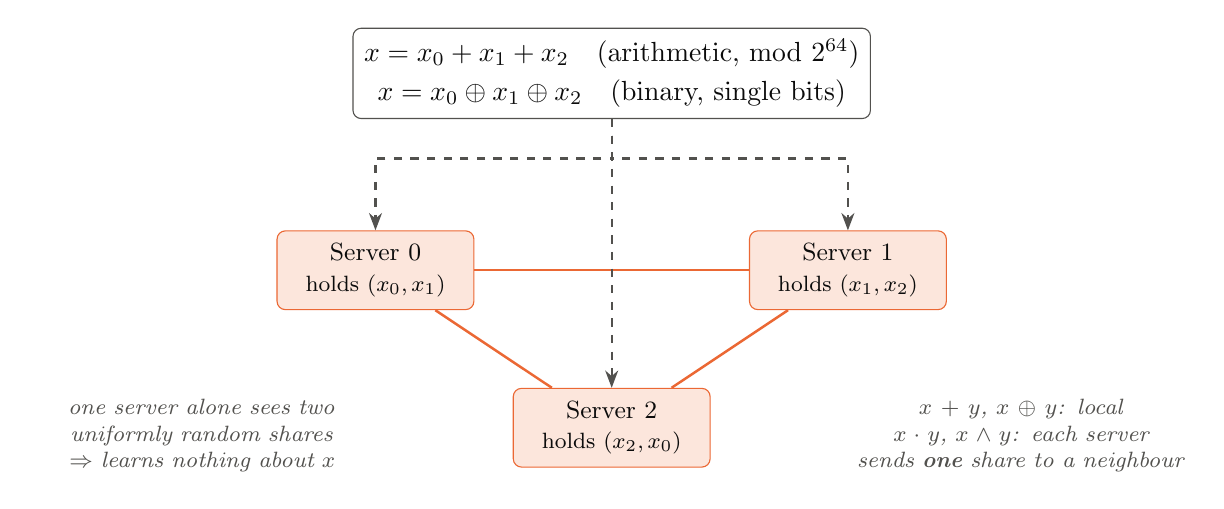
\begin{tikzpicture}
  \node[box, font=\normalsize] (x) at (0, 2.5)
    {$x = x_0 + x_1 + x_2$\quad(arithmetic, mod $2^{64}$)\\[2pt]
     $x = x_0 \oplus x_1 \oplus x_2$\quad(binary, single bits)};

  \node[server] (p0) at (-3.0, 0)   {Server 0\\\footnotesize holds $(x_0, x_1)$};
  \node[server] (p1) at ( 3.0, 0)   {Server 1\\\footnotesize holds $(x_1, x_2)$};
  \node[server] (p2) at ( 0, -2.0)  {Server 2\\\footnotesize holds $(x_2, x_0)$};
  \draw[link] (p0) -- (p1);
  \draw[link] (p1) -- (p2);
  \draw[link] (p2) -- (p0);

  \draw[arr, dashed] (x.south) -- ++(0,-0.5) -| (p0.north);
  \draw[arr, dashed] (x.south) -- ++(0,-0.5) -| (p1.north);
  \draw[arr, dashed] (x.south) -- (p2.north);

  \node[note, text width=4.2cm] at (-5.2, -2.1) {one server alone sees two\\
    uniformly random shares\\$\Rightarrow$ learns nothing about $x$};
  \node[note, text width=4.2cm] at (5.2, -2.1) {$x + y$, $x \oplus y$: local\\
    $x \cdot y$, $x \wedge y$: each server\\sends \textbf{one} share to a neighbour};
\end{tikzpicture}
}
  \caption{3-party replicated secret sharing. Each server holds two of the three shares; one
           server alone sees only random values. Local operations are free; each multiplication
           (AND) costs one share sent per server.}
  \label{fig:replicated}
\end{figure}

\paragraph{MP-SPDZ.}
MP-SPDZ~\cite{mpspdz} compiles a high-level Python-like program (\code{.mpc}) into bytecode that
any of its protocols can execute. It reports the exact number of multiplications (``triples''),
rounds and opened values the program needs, which we use both to audit the output boundary and to
validate our cost model. It also implements malicious variants of the same protocols (security
with abort)~\cite{lindellnof17,furukawa17}, which we use in \cref{sec:security-eval}.

\paragraph{The bit-slice maximum.}
Kurosawa and Ogata~\cite{ko02} find the maximum of $n$ hidden $k$-bit numbers by one scan from the
most significant bit down, keeping a mask $S$ of bidders who could still hold the maximum. At each
bit, if some survivor has a 1, all survivors with a 0 are eliminated. Only AND and OR on bits are
needed, so the scan can run in any MPC that supports them.

% ==============================================================================
\section{System Design}
\label{sec:design}

\subsection{Architecture and threat model}

\Cref{fig:architecture} shows the system. Each bidder secret-shares its bid and sends share $p$
to server $p$. The three servers run the auction circuit under MP-SPDZ and open only the winner
and the price. The threat model is that of the survey (\S7): servers and bidders follow the
protocol (semi-honest) but may try to learn from what they see; at most one server is corrupted;
collusion of two servers is outside the model.

\begin{figure}[H]
  \centering
  \resizebox{0.92\linewidth}{!}{% System architecture: bidders secret-share their bids to three servers,
% which jointly compute and open only the winner and the price.
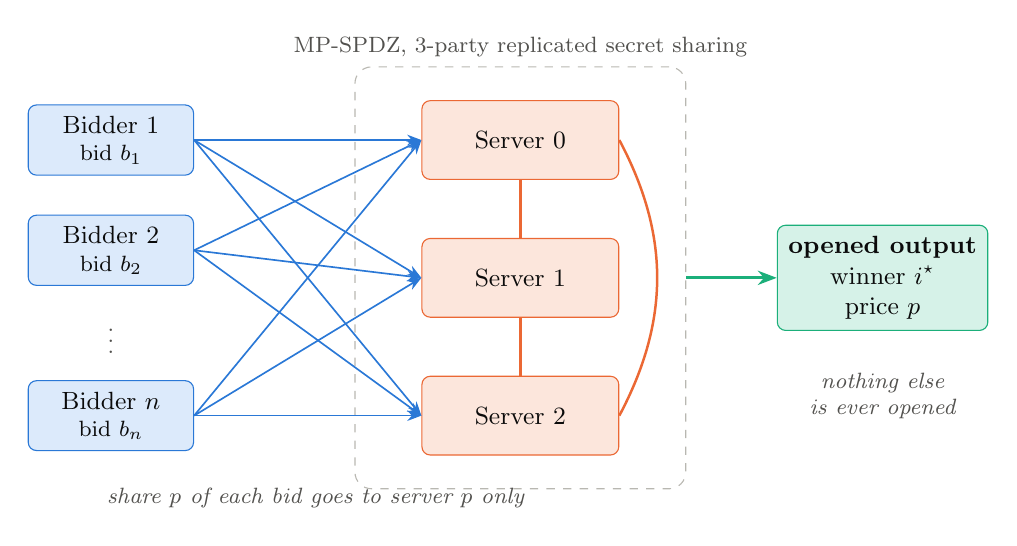
\begin{tikzpicture}[node distance=0.5cm]
  % bidders
  \node[bidder] (b1) at (0, 2.1) {Bidder 1\\[-1pt]\footnotesize bid $b_1$};
  \node[bidder] (b2) at (0, 0.7) {Bidder 2\\[-1pt]\footnotesize bid $b_2$};
  \node[lbl]    (bd) at (0, -0.35) {$\vdots$};
  \node[bidder] (bn) at (0, -1.4) {Bidder $n$\\[-1pt]\footnotesize bid $b_n$};

  % servers
  \node[server] (s0) at (5.2, 2.1)  {Server 0};
  \node[server] (s1) at (5.2, 0.35) {Server 1};
  \node[server] (s2) at (5.2, -1.4) {Server 2};
  \draw[link] (s0.east) to[bend left=28] (s2.east);
  \draw[link] (s0) -- (s1);
  \draw[link] (s1) -- (s2);

  % shares
  \foreach \b in {b1, b2, bn} {
    \foreach \s/\p in {s0/0, s1/1, s2/2} {
      \draw[sharearr] (\b.east) -- (\s.west);
    }
  }
  \node[note] at (2.6, -2.45) {share $p$ of each bid goes to server $p$ only};

  % MPC region
  \begin{scope}[on background layer]
    \node[region, fit=(s0)(s1)(s2), inner xsep=24pt, inner ysep=12pt,
          label={[lbl]above:MP-SPDZ, 3-party replicated secret sharing}] (mpc) {};
  \end{scope}

  % output
  \node[outbox, minimum width=2.6cm] (out) at (9.8, 0.35)
    {\textbf{opened output}\\winner $i^\star$\\price $p$};
  \draw[outarr] (mpc.east |- out) -- (out.west);
  \node[note] at (9.8, -1.15) {nothing else\\is ever opened};
\end{tikzpicture}
}
  \caption{System architecture. Bidders are not servers: they only send random-looking shares.
           The servers compute jointly and open only the winner $i^\star$ and price $p$.}
  \label{fig:architecture}
\end{figure}

\subsection{Input sharing}
\label{sec:input}

Bidders share their bids locally (\code{auction/sharing.py}). Each bidder first writes its bid in
binary, which is trivial for the bidder, and then shares every bit separately:
\begin{itemize}
  \item \textbf{arithmetic domain}: each bit $b_i[j]$ is split into three additive shares modulo
        $2^{64}$;
  \item \textbf{binary domain}: the bid is split into three $k$-bit XOR shares.
\end{itemize}
The servers therefore receive shares of the bits directly and never have to extract bits from a
shared number.
Each server feeds its shares to MP-SPDZ as private inputs, and the program adds (or XORs) the three
inputs \emph{inside} the computation, so the reconstructed bid exists only in shared form. Server
$p$'s input file holds a $k \times n$ matrix of shares in bit-major order (row $j$ holds bit $j$ of
every bidder), so each bit position is read as one contiguous vector.

\subsection{The oblivious bit-slice scan}
\label{sec:scan}

The survey describes the update step as a branch on the check bit. A branch on secret data would
leak it, so we write the step as pure arithmetic on shared 0/1 values (\cref{alg:scan},
\cref{fig:bitcircuit}). Let $t_i = S_i \cdot b_i[j]$ (survivor $i$ has a 1 at bit $j$) and
$c_j = \bigvee_i t_i$. The required update $S_i \leftarrow S_i \cdot (1 - c_j(1 - b_i[j]))$
expands to
\begin{equation}
  S_i' \;=\; S_i - c_j\,(S_i - t_i),
  \label{eq:update}
\end{equation}
which reuses $t_i$ and needs one multiplication per bidder instead of two. The $n$-input OR is a
balanced tree of $x \vee y = 1 - (1-x)(1-y)$, with $n-1$ ANDs in $\lceil\log_2 n\rceil$ rounds
(\cref{fig:ortree}). Since every $c_j$ is a bit of the maximum, the maximum itself is
$\sum_j c_j 2^j$ at no extra cost.

\begin{algo}[t]
\begin{lstlisting}
Input: shared bits $b_i[j]$ for bidders $i = 0..n-1$, bits $j = 0..k-1$
$S \leftarrow (1, \dots, 1)$                                  $\textit{// all bidders survive}$
for $j = k-1$ downto $0$:
    $t \leftarrow S \cdot b[j]$                                 $\textit{// n ANDs, vectorised}$
    $c_j \leftarrow 1 - \prod_i (1 - t_i)$                        $\textit{// OR tree: n-1 ANDs}$
    $S \leftarrow S - c_j\,(S - t)$                             $\textit{// n ANDs, Eq. (1)}$
return mask $S$, maximum bits $(c_{k-1}, \dots, c_0)$
\end{lstlisting}
\caption{Oblivious bit-slice scan (\code{bitslice\_scan} in \code{mpc/auction.mpc}). No step
depends on a secret value, so the compiled circuit is fixed by $n$, $k$ and the mechanism.}
\label{alg:scan}
\end{algo}

\begin{figure}[t]
  \centering
  \resizebox{\linewidth}{!}{% One step of the oblivious scan (bit position j); all wires carry secret shares.
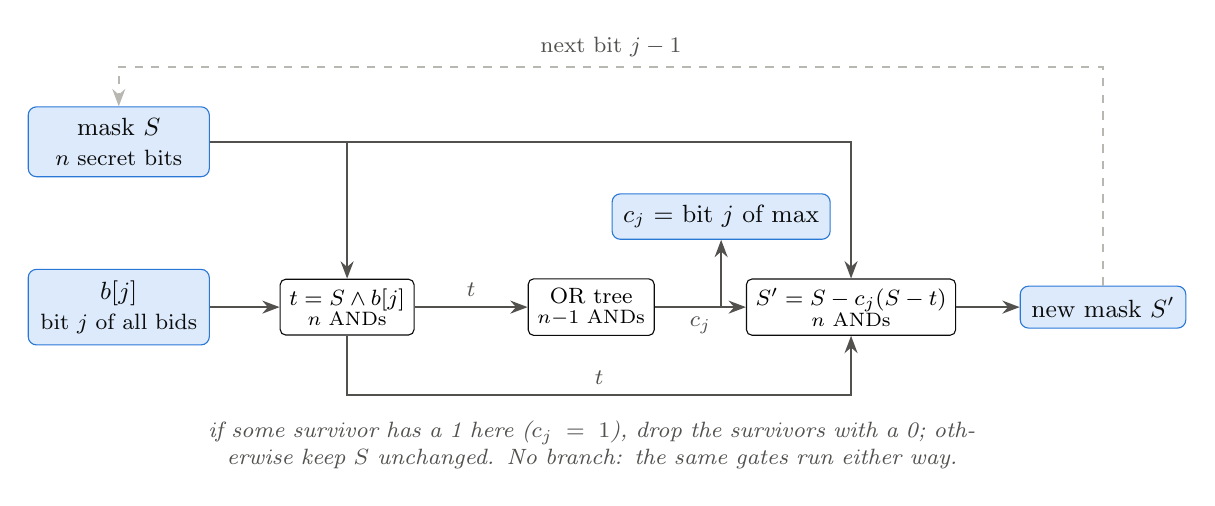
\begin{tikzpicture}
  \node[secret, minimum width=2.3cm] (S) at (0, 1.5) {mask $S$\\\footnotesize $n$ secret bits};
  \node[secret, minimum width=2.3cm] (b) at (0, -0.6) {$b[j]$\\\footnotesize bit $j$ of all bids};

  \node[gate] (and) at (2.9, -0.6) {$t = S \wedge b[j]$\\[-2pt]\scriptsize $n$ ANDs};
  \node[gate] (or) at (6.0, -0.6) {OR tree\\[-2pt]\scriptsize $n{-}1$ ANDs};
  \node[gate] (upd) at (9.3, -0.6) {$S' = S - c_j(S - t)$\\[-2pt]\scriptsize $n$ ANDs};
  \node[secret, minimum width=1.9cm] (Sn) at (12.5, -0.6) {new mask $S'$};
  \node[secret] (cj) at (7.65, 0.55) {$c_j$ = bit $j$ of max};

  \draw[arr] (b) -- (and);
  \draw[arr] (S.east) -| (and.north);
  \draw[arr] (S.east) -| (upd.north);
  \draw[arr] (and) -- node[lbl, above] {$t$} (or);
  \draw[arr] (or) -- node[lbl, below] {$c_j$} (upd);
  \draw[arr] (7.65, -0.6) -- (cj.south);
  \draw[arr] (and.south) -- ++(0, -0.75) -| node[lbl, pos=0.25, above] {$t$} (upd.south);
  \draw[arr] (upd) -- (Sn);
  \draw[arr, dashed, draw=vline] (Sn.north) |- node[lbl, pos=0.75, above] {next bit $j-1$}
      ($(S.north)+(0,0.5)$) -- (S.north);

  \node[note, text width=11cm] at (6.0, -2.35)
    {if some survivor has a 1 here ($c_j = 1$), drop the survivors with a 0;
     otherwise keep $S$ unchanged. No branch: the same gates run either way.};
\end{tikzpicture}
}
  \caption{One step of the scan. All wires carry secret shares; the same gates run whatever the
           data, so the step is oblivious.}
  \label{fig:bitcircuit}
\end{figure}

\begin{figure}[t]
  \centering
  \resizebox{0.78\linewidth}{!}{% Log-depth n-input OR used at every bit position (n = 8 shown).
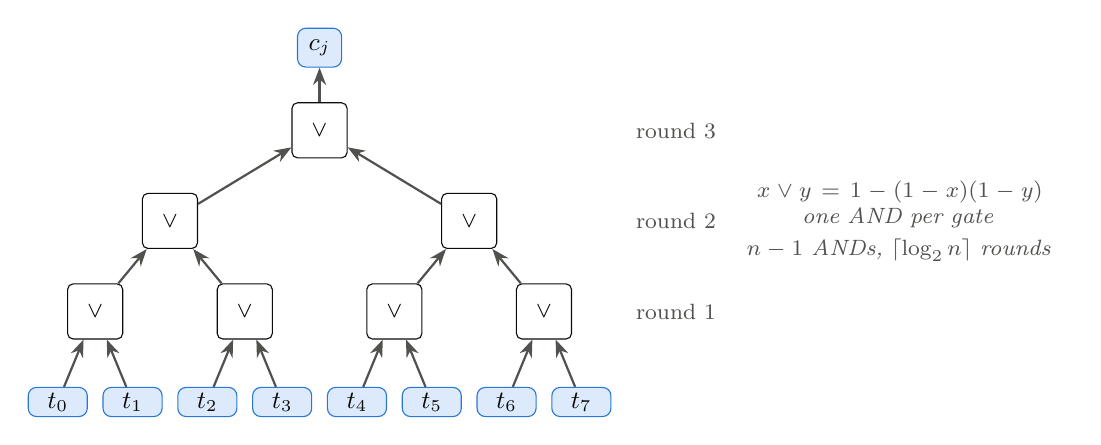
\begin{tikzpicture}[x=0.95cm, y=1.0cm]
  \foreach \i in {0,...,7}
    \node[secret, minimum width=0.75cm, inner sep=2pt] (t\i) at (\i, 0) {$t_{\i}$};
  \foreach \i/\a/\b in {0/0/1, 1/2/3, 2/4/5, 3/6/7} {
    \node[gate, minimum width=0.7cm] (l\i) at ({\a+0.5}, 1.15) {$\vee$};
    \draw[arr] (t\a) -- (l\i); \draw[arr] (t\b) -- (l\i);
  }
  \foreach \i/\a/\b in {0/0/1, 1/2/3} {
    \node[gate, minimum width=0.7cm] (m\i) at ({2*\a+1.5}, 2.3) {$\vee$};
    \draw[arr] (l\a) -- (m\i); \draw[arr] (l\b) -- (m\i);
  }
  \node[gate, minimum width=0.7cm] (r) at (3.5, 3.45) {$\vee$};
  \draw[arr] (m0) -- (r); \draw[arr] (m1) -- (r);
  \node[secret] (c) at (3.5, 4.5) {$c_j$};
  \draw[arr] (r) -- (c);

  \foreach \y/\lab in {1.15/round 1, 2.3/round 2, 3.45/round 3}
    \node[lbl, anchor=west] at (7.6, \y) {\lab};
  \node[note, anchor=west, text width=4.2cm] at (8.9, 2.3)
    {$x \vee y = 1 - (1-x)(1-y)$\\one AND per gate\\[2pt]$n-1$ ANDs, $\lceil\log_2 n\rceil$ rounds};
\end{tikzpicture}
}
  \caption{The $n$-input OR computed at every bit position ($n=8$).}
  \label{fig:ortree}
\end{figure}

\Cref{fig:worked} replays the survey's worked example ($A = 11$, $B = 13$, $C = 9$) through
\cref{alg:scan}. It also corrects Table~1 of the survey, which printed the mask after bits 1 and 0
as $\{\}$: when no survivor has a 1 the mask is carried forward, so it stays $\{B\}$. Our test
suite checks this trace exactly (\code{test\_worked\_example\_trace}).

\begin{figure}[H]
  \centering
  \resizebox{0.85\linewidth}{!}{% Bit-slice scan on A = 11, B = 13, C = 9 (corrected Table 1 of the lit survey).
% Blue cells: bidder still a survivor when that bit is examined.
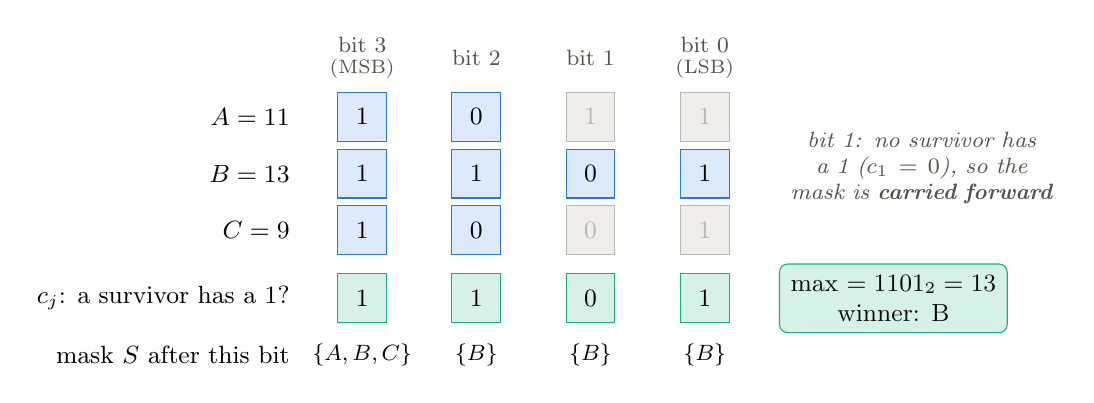
\begin{tikzpicture}[x=1.45cm, y=0.72cm]
  % header
  \foreach \c/\lab in {0/{bit 3\\[-2pt]\scriptsize(MSB)}, 1/{bit 2}, 2/{bit 1}, 3/{bit 0\\[-2pt]\scriptsize(LSB)}}
    \node[lbl, align=center] at (\c, 1.05) {\lab};
  % rows: name, value, bits (MSB first), survivor flags per column
  \foreach \r/\name/\val/\bits/\alive in {
      0/A/11/{1,0,1,1}/{1,1,0,0},
      1/B/13/{1,1,0,1}/{1,1,1,1},
      2/C/9/{1,0,0,1}/{1,1,0,0}} {
    \node[font=\small, anchor=east] at (-0.55, -\r) {$\name = \val$};
    \foreach \bit [count=\c from 0] in \bits {
      \pgfmathsetmacro{\a}{{\alive}[\c]}
      \ifdim \a pt > 0.5pt
        \node[bitcell, fill=vbluebg, draw=vblue] at (\c, -\r) {\bit};
      \else
        \node[bitcell, fill=vlight, text=vline] at (\c, -\r) {\bit};
      \fi
    }
  }
  % c_j row and mask row
  \node[font=\small, anchor=east] at (-0.55, -3.2) {$c_j$: a survivor has a 1?};
  \node[font=\small, anchor=east] at (-0.55, -4.2) {mask $S$ after this bit};
  \foreach \c/\cj/\mask in {0/1/{\{A,B,C\}}, 1/1/{\{B\}}, 2/0/{\{B\}}, 3/1/{\{B\}}} {
    \node[bitcell, fill=vaquabg, draw=vaqua] at (\c, -3.2) {\cj};
    \node[font=\footnotesize] at (\c, -4.2) {$\mask$};
  }
  \node[outbox, anchor=west] at (3.65, -3.2) {max $= 1101_2 = 13$\\winner: B};
  \node[note, anchor=west, text width=3.4cm] at (3.65, -0.9)
    {bit 1: no survivor has a 1 ($c_1 = 0$), so the mask is \textbf{carried forward}};
\end{tikzpicture}
}
  \caption{The scan on the survey's example. Blue cells: bidder still a survivor at that bit.
           This corrects the last two rows of Table~1 in the survey.}
  \label{fig:worked}
\end{figure}

\subsection{Ties: an oblivious lowest-index winner}

When several bidders share the maximum, the final mask contains all of them. Opening it would
reveal who tied, a leak the privacy target forbids. Instead we keep only the first survivor,
$w_i = S_i \prod_{l<i} (1 - S_l)$, using a Hillis--Steele prefix product in $\lceil\log_2 n\rceil$
rounds, and open only $\sum_i i \cdot w_i$ (\cref{fig:tiebreak}). The tournament baseline uses the
same tie rule, so all programs produce identical outputs.

\begin{figure}[H]
  \centering
  \resizebox{0.8\linewidth}{!}{% Oblivious lowest-index tie-break: keep only the first survivor.
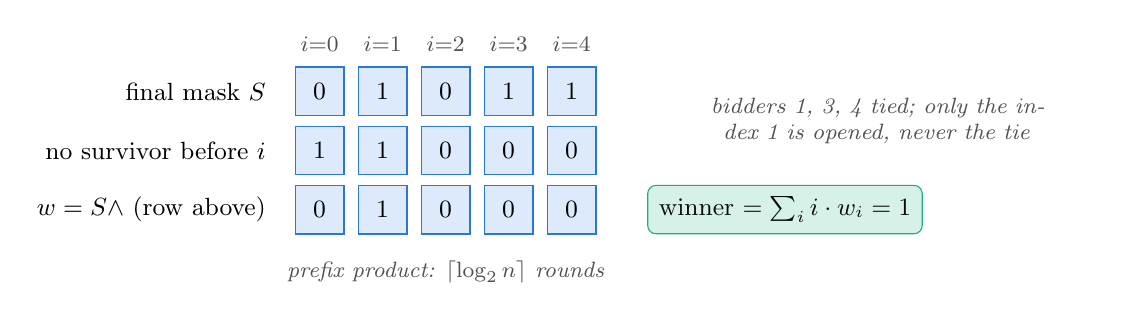
\begin{tikzpicture}[x=0.8cm, y=0.75cm]
  \foreach \i in {0,...,4} \node[lbl] at (\i, 0.8) {$i{=}\i$};
  \foreach \r/\lab/\vals/\col in {
      0/{final mask $S$}/{0,1,0,1,1}/vblue,
      1/{no survivor before $i$}/{1,1,0,0,0}/vblue,
      2/{$w = S \wedge$ (row above)}/{0,1,0,0,0}/vblue} {
    \node[font=\small, anchor=east] at (-0.7, -\r) {\lab};
    \foreach \v [count=\c from 0] in \vals
      \node[bitcell, fill=vbluebg, draw=\col] at (\c, -\r) {\v};
  }
  \node[outbox, anchor=west] at (5.2, -2) {winner $= \sum_i i\cdot w_i = 1$};
  \node[note, anchor=west, text width=5.6cm] at (5.2, -0.5)
    {bidders 1, 3, 4 tied; only the index 1 is opened, never the tie};
  \node[note] at (2, -3.05) {prefix product: $\lceil\log_2 n\rceil$ rounds};
\end{tikzpicture}
}
  \caption{Oblivious lowest-index tie-break: three bidders tie, but only the index of the first is
           opened.}
  \label{fig:tiebreak}
\end{figure}

\subsection{The Vickrey extension}

For the second price we remove the winner obliviously and scan again (\cref{fig:vickrey}): every
bit of the winner is zeroed with $b_i[j] \leftarrow b_i[j]\,(1 - w_i)$, and the new maximum is the
second-highest bid. The first-scan bits $c_j$, which encode the winning bid, are never opened.
Two edge cases come out right without special handling: tied top bids give a price equal to the top
bid, and a single bidder pays 0. The cost roughly doubles.

\begin{figure}[H]
  \centering
  \resizebox{0.95\linewidth}{!}{% Vickrey pipeline: two scans; the first-scan maximum is never opened.
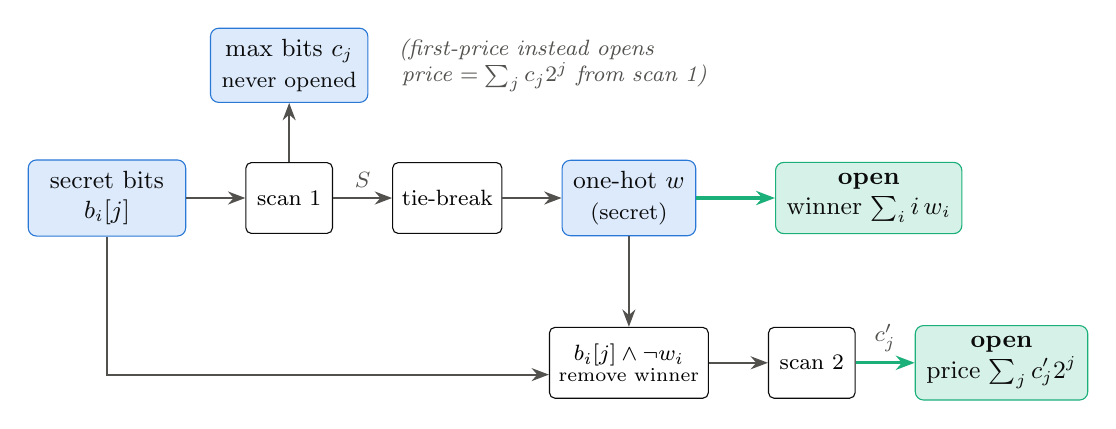
\begin{tikzpicture}[node distance=0.55cm and 0.75cm]
  \node[secret, minimum width=2.0cm] (B) {secret bits\\$b_i[j]$};
  \node[gate, right=of B, minimum height=0.9cm] (s1) {scan 1};
  \node[gate, right=of s1, minimum height=0.9cm] (tb) {tie-break};
  \node[secret, right=of tb] (w) {one-hot $w$\\\footnotesize (secret)};
  \node[outbox, right=1.0cm of w] (win) {\textbf{open}\\winner $\sum_i i\, w_i$};

  \node[secret, above=0.75cm of s1] (c1) {max bits $c_j$\\\footnotesize never opened};
  \node[gate, below=1.15cm of w, minimum height=0.9cm] (zero) {$b_i[j] \wedge \lnot w_i$\\[-2pt]\scriptsize remove winner};
  \node[gate, right=of zero, minimum height=0.9cm] (s2) {scan 2};
  \node[outbox, right=0.75cm of s2] (price) {\textbf{open}\\price $\sum_j c'_j 2^j$};

  \draw[arr] (B) -- (s1);
  \draw[arr] (s1) -- node[lbl, above] {$S$} (tb);
  \draw[arr] (tb) -- (w);
  \draw[outarr] (w) -- (win);
  \draw[arr] (s1) -- (c1);
  \draw[arr] (w) -- (zero);
  \draw[arr] (B.south) |- ($(zero.west)+(0,-0.15)$);
  \draw[arr] (zero) -- (s2);
  \draw[outarr] (s2) -- node[lbl, above] {$c'_j$} (price);

  \node[note, right=0.3cm of c1, text width=5.2cm, align=left] {(first-price instead opens\\price $= \sum_j c_j 2^j$ from scan 1)};
\end{tikzpicture}
}
  \caption{Vickrey pipeline. Secret values in blue, opened values in green. Only the winner index
           and the second-scan maximum are opened.}
  \label{fig:vickrey}
\end{figure}

\subsection{The binary-domain instantiation}
\label{sec:binary}

The scan only ever combines single bits, yet in $\Z_{2^{64}}$ each AND is a full 64-bit ring
multiplication. \code{mpc/auction\_bin.mpc} runs the identical circuit on XOR-shared bits under
MP-SPDZ's \code{replicated-bin} protocol (\cref{fig:domains}). Bit $j$ of all $n$ bidders is
packed into one $n$-bit word, so each line of \cref{alg:scan} is a single word-wide operation, and
\cref{eq:update} becomes $S' = S \oplus (c_j \wedge (S \oplus t))$. XOR and NOT are free and each
AND costs one bit per server. The winner index needs no arithmetic: since $w$ is one-hot, bit $m$
of the index is the XOR of the $w_i$ whose index has bit $m$ set.

\begin{figure}[H]
  \centering
  \resizebox{0.95\linewidth}{!}{% Arithmetic vs binary domain: same circuit, different cost per AND.
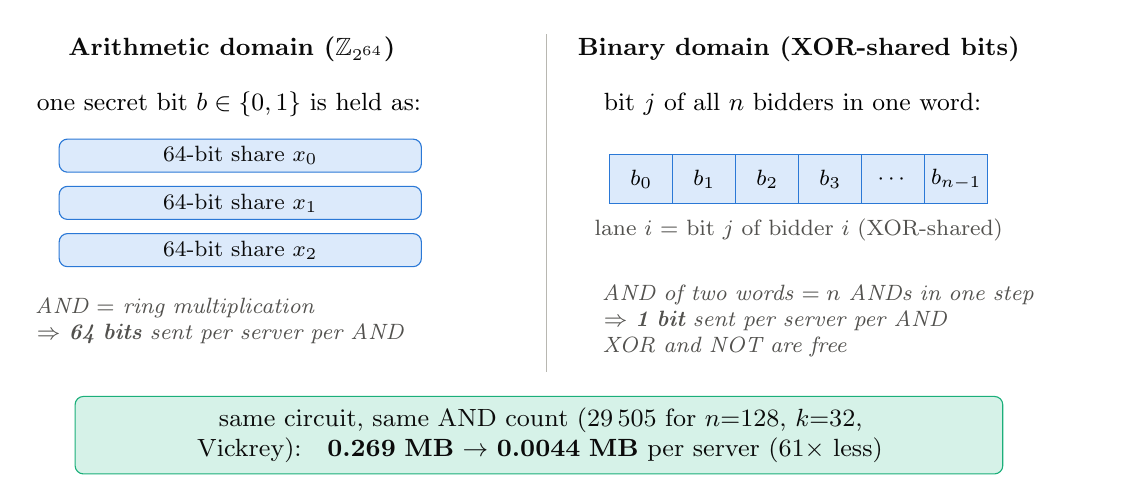
\begin{tikzpicture}
  % ---- arithmetic panel
  \node[lbl, font=\small\bfseries, text=vink] at (2.6, 2.9) {Arithmetic domain ($\mathbb{Z}_{2^{64}}$)};
  \node[font=\small, anchor=west] at (0, 2.2) {one secret bit $b \in \{0,1\}$ is held as:};
  \foreach \i/\y in {0/1.55, 1/0.95, 2/0.35} {
    \node[secret, minimum width=4.6cm, minimum height=0.42cm, inner sep=1pt, anchor=west]
      at (0.4, \y) {\footnotesize 64-bit share $x_{\i}$};
  }
  \node[note, anchor=west, text width=5.3cm, align=left] at (0, -0.55)
    {AND $=$ ring multiplication\\$\Rightarrow$ \textbf{64 bits} sent per server per AND};

  % ---- binary panel
  \begin{scope}[xshift=7.2cm]
    \node[lbl, font=\small\bfseries, text=vink] at (2.6, 2.9) {Binary domain (XOR-shared bits)};
    \node[font=\small, anchor=west] at (0, 2.2) {bit $j$ of all $n$ bidders in one word:};
    \foreach \i/\lab in {0/$b_0$, 1/$b_1$, 2/$b_2$, 3/$b_3$, 4/$\cdots$, 5/$b_{n-1}$} {
      \node[bitcell, fill=vbluebg, draw=vblue, minimum width=0.8cm] at ({0.8*\i+0.6}, 1.25) {\footnotesize \lab};
    }
    \node[lbl] at (2.6, 0.6) {lane $i$ = bit $j$ of bidder $i$ (XOR-shared)};
    \node[note, anchor=west, text width=6.2cm, align=left] at (0, -0.55)
      {AND of two words $= n$ ANDs in one step\\$\Rightarrow$ \textbf{1 bit} sent per server per AND\\XOR and NOT are free};
  \end{scope}

  \draw[draw=vline] (6.6, -1.2) -- (6.6, 3.1);
  \node[outbox, text width=11.5cm] at (6.5, -2.0)
    {same circuit, same AND count (29\,505 for $n{=}128$, $k{=}32$, Vickrey):\quad
     \textbf{0.269 MB} $\to$ \textbf{0.0044 MB} per server (61$\times$ less)};
\end{tikzpicture}
}
  \caption{Arithmetic versus binary domain. The circuit and its AND count are identical; only the
           cost of each AND changes.}
  \label{fig:domains}
\end{figure}

\subsection{Baseline: a tournament of secure comparisons}

To evaluate the bit-slice approach against the ``naive'' approach of survey \S5.1, we implement a
knockout tournament (\cref{fig:tournament}) using MP-SPDZ's built-in secure comparison, in both
domains (\code{baseline\_tournament.mpc}, \code{baseline\_tournament\_bin.mpc}). Each level compares
neighbouring brackets in one vectorised step and multiplexes the running maximum, runner-up and
index. Neighbours are paired as $(2i, 2i+1)$ and the right bracket wins only on a strict $>$, so the
lowest index wins ties.

\begin{figure}[H]
  \centering
  \resizebox{0.8\linewidth}{!}{% Baseline: knockout tournament of secure comparisons (n = 8).
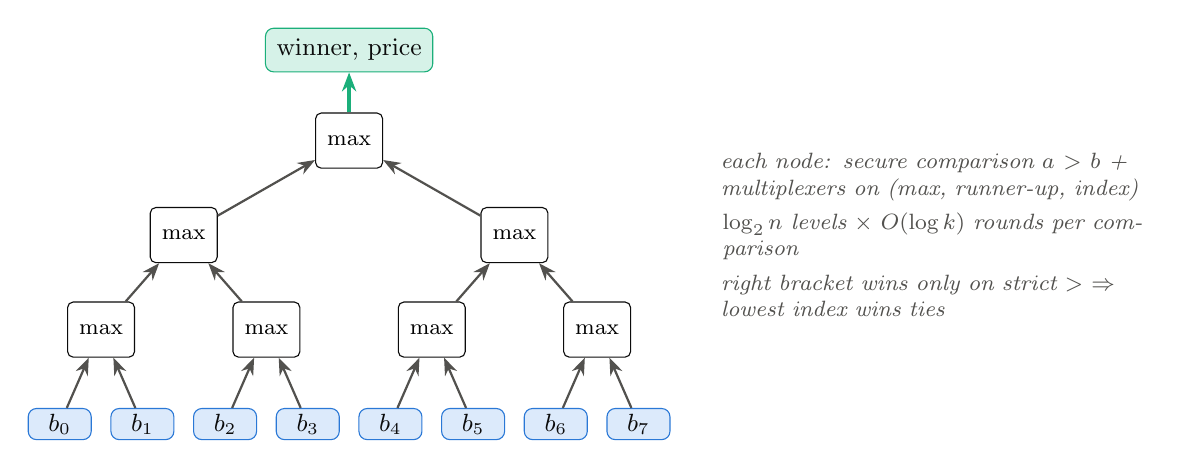
\begin{tikzpicture}[x=1.05cm, y=1.0cm]
  \foreach \i in {0,...,7}
    \node[secret, minimum width=0.8cm, inner sep=2pt] (b\i) at (\i, 0) {$b_{\i}$};
  \foreach \i/\a/\b in {0/0/1, 1/2/3, 2/4/5, 3/6/7} {
    \node[gate, minimum width=0.85cm] (l\i) at ({\a+0.5}, 1.2) {$\max$};
    \draw[arr] (b\a) -- (l\i); \draw[arr] (b\b) -- (l\i);
  }
  \foreach \i/\a/\b in {0/0/1, 1/2/3} {
    \node[gate, minimum width=0.85cm] (m\i) at ({2*\a+1.5}, 2.4) {$\max$};
    \draw[arr] (l\a) -- (m\i); \draw[arr] (l\b) -- (m\i);
  }
  \node[gate, minimum width=0.85cm] (r) at (3.5, 3.6) {$\max$};
  \draw[arr] (m0) -- (r); \draw[arr] (m1) -- (r);
  \node[outbox] (o) at (3.5, 4.75) {winner, price};
  \draw[outarr] (r) -- (o);

  \node[note, anchor=west, text width=5.3cm, align=left] at (7.9, 2.4)
    {each node: secure comparison $a > b$ + multiplexers on (max, runner-up, index)\\[3pt]
     $\log_2 n$ levels $\times$ $O(\log k)$ rounds per comparison\\[3pt]
     right bracket wins only on strict $>$ $\Rightarrow$ lowest index wins ties};
\end{tikzpicture}
}
  \caption{Comparison-tournament baseline ($n=8$).}
  \label{fig:tournament}
\end{figure}

% ==============================================================================
\section{Security Analysis}
\label{sec:security}

\paragraph{Ideal functionality.}
$\mathcal{F}_\text{auction}$ receives every bid and returns $(i^\star, p)$, the lowest-index
highest bidder and its price under the chosen rule. We argue that the protocol securely realises
$\mathcal{F}_\text{auction}$ against a semi-honest adversary statically corrupting one server.

\paragraph{Simulation sketch.}
The corrupted server's view consists of three parts, each of which a simulator given only
$(i^\star, p)$ can reproduce.
\begin{enumerate}
  \item \emph{Inputs.} For every bid (or bit), it holds one share $s_p$ of
        $b = s_0 + s_1 + s_2$, where the bidder chose two shares uniformly at random. Any single
        share is therefore uniform on $\Z_{2^{64}}$ (or on $k$-bit strings for XOR sharing) and
        independent of $b$, so the simulator samples random values. Our test suite checks this
        empirically with a $\chi^2$ test (\code{test\_single\_share\_looks\_uniform}).
  \item \emph{Computation.} The program is a fixed composition of local operations and secure
        multiplications of the replicated protocol, each simulatable for one corrupted
        party~\cite{araki16}. Control flow, number of rounds and message sizes depend only on the
        public parameters $(n, k, \text{mechanism})$, so nothing leaks through them.
  \item \emph{Outputs.} Exactly two values are opened. Given $(i^\star, p)$ the simulator chooses
        the honest parties' opening messages consistent with them.
\end{enumerate}
By sequential composition, the corrupted server learns nothing beyond $(i^\star, p)$.

\paragraph{Reveal audit.}
\code{auction/audit.py} recompiles the programs and checks MP-SPDZ's count of opened values. The
arithmetic program opens exactly 2 integers and the binary program reveals exactly two words, for
every $n$ and both mechanisms. The tournament baseline, by contrast, also opens masked values inside
MP-SPDZ's comparison protocol.

\begin{table}[H]
\centering\small
\begin{tabularx}{\linewidth}{@{}l>{\raggedright\arraybackslash}X@{}}
\toprule
\textbf{Party} & \textbf{What it sees} \\
\midrule
Bidder & its own bid, its own shares, and the public output $(i^\star, p)$ \\
One server & uniformly random shares of every bid, protocol messages that are themselves fresh
             random shares, and $(i^\star, p)$ \\
Network observer & encrypted channels (MP-SPDZ uses TLS between servers); at most shares \\
Two colluding servers & \emph{outside the model}: together they can reconstruct every bid \\
\bottomrule
\end{tabularx}
\caption{Per-party view, matching the threat model of the survey (\S7.2).}
\label{tab:views}
\end{table}

\paragraph{Inherent leakage.}
As stated in the survey, information implied by the output itself is not a leak: a first-price
outcome reveals that every losing bid is at most $p$; a Vickrey outcome reveals that $p$ is the
second-highest bid. Ranks, orderings and ties among losers stay hidden.

\paragraph{Limitations of the guarantee.}
Bidders are trusted to submit well-formed inputs: a malicious bidder could share a ``bit'' equal
to 2 and corrupt the result. Computing and opening $b_i[j](1 - b_i[j])$, which is 0 for every
valid bit, would detect this at the cost of $nk$ extra multiplications. Under the malicious protocols of \cref{sec:security-eval}, the \emph{computation} is
secure with abort against one malicious server, but a malicious server could still substitute its
input share of a bid, since bidder shares are not authenticated. MP-SPDZ's client-input protocol,
in which bidders mask their inputs with preprocessed random values, would close this gap.

% ==============================================================================
\section{Implementation}
\label{sec:impl}

The code base is organised into the four components declared in the mid-term report
(\cref{fig:components}); \cref{fig:workflow} shows how they interact in one run.

\begin{figure}[H]
  \centering
  \resizebox{\linewidth}{!}{% Code components and team ownership (as declared in the mid-term report).
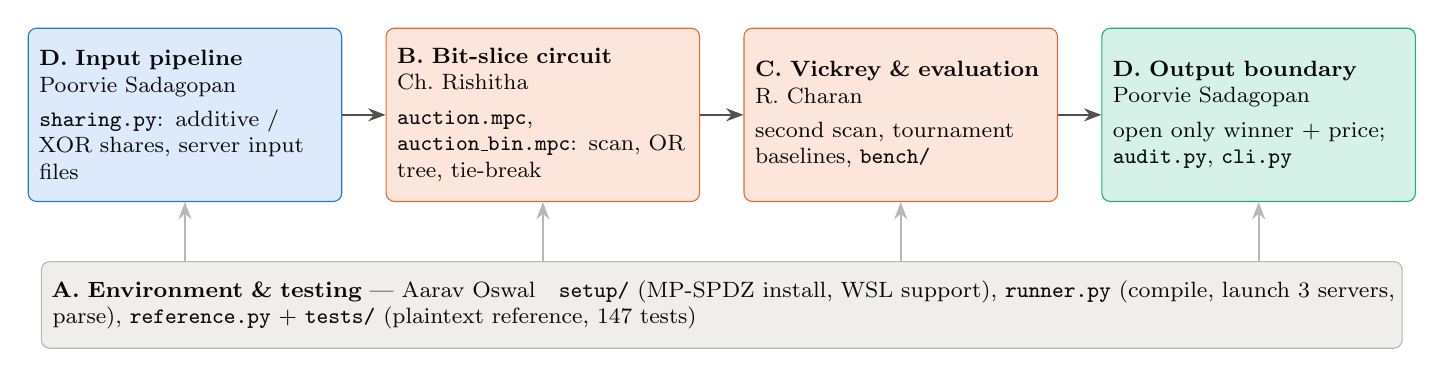
\begin{tikzpicture}[node distance=0.5cm and 0.55cm]
  \tikzset{comp/.style={box, text width=3.7cm, minimum height=2.2cm, align=left, font=\footnotesize}}
  \node[comp, fill=vbluebg, draw=vblue] (d1) {\textbf{D. Input pipeline}\\Poorvie Sadagopan\\[3pt]
    \texttt{sharing.py}: additive / XOR shares, server input files};
  \node[comp, fill=vorangebg, draw=vorange, right=of d1] (b) {\textbf{B. Bit-slice circuit}\\Ch.\ Rishitha\\[3pt]
    \texttt{auction.mpc}, \texttt{auction\_bin.mpc}: scan, OR tree, tie-break};
  \node[comp, fill=vorangebg, draw=vorange, right=of b] (c) {\textbf{C. Vickrey \& evaluation}\\R.\ Charan\\[3pt]
    second scan, tournament baselines, \texttt{bench/}};
  \node[comp, fill=vaquabg, draw=vaqua, right=of c] (d2) {\textbf{D. Output boundary}\\Poorvie Sadagopan\\[3pt]
    open only winner + price; \texttt{audit.py}, \texttt{cli.py}};
  \draw[arr] (d1) -- (b); \draw[arr] (b) -- (c); \draw[arr] (c) -- (d2);

  \node[comp, fill=vlight, draw=vline, text width=17.0cm, minimum height=1.1cm,
        below=0.75cm of $(b.south)!0.5!(c.south)$] (a)
    {\textbf{A. Environment \& testing} --- Aarav Oswal\quad
     \texttt{setup/} (MP-SPDZ install, WSL support), \texttt{runner.py} (compile, launch 3 servers, parse),
     \texttt{reference.py} + \texttt{tests/} (plaintext reference, 147 tests)};
  \foreach \x in {d1, b, c, d2} \draw[arr, draw=vline] (a.north -| \x.south) -- (\x.south);
\end{tikzpicture}
}
  \caption{Code components and their owners, as declared in the mid-term report.}
  \label{fig:components}
\end{figure}

\begin{figure}[H]
  \centering
  \resizebox{0.95\linewidth}{!}{% End-to-end workflow of one auction run, with the source file for each step.
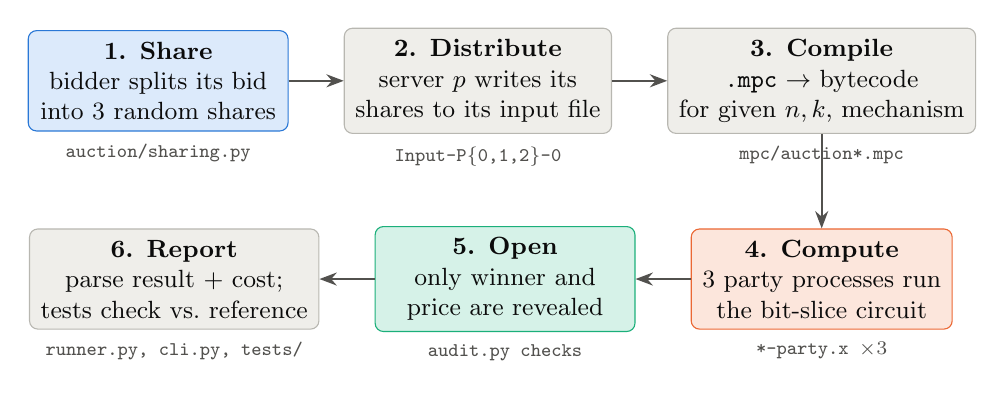
\begin{tikzpicture}[node distance=0.55cm and 0.7cm]
  \node[stepbox, secret] (s1) {\textbf{1. Share}\\bidder splits its bid\\into 3 random shares};
  \node[stepbox, plain, right=of s1] (s2) {\textbf{2. Distribute}\\server $p$ writes its\\shares to its input file};
  \node[stepbox, plain, right=of s2] (s3) {\textbf{3. Compile}\\\texttt{.mpc} $\to$ bytecode\\for given $n,k$, mechanism};

  \node[stepbox, server, below=1.2cm of s3] (s4) {\textbf{4. Compute}\\3 party processes run\\the bit-slice circuit};
  \node[stepbox, outbox, left=of s4] (s5) {\textbf{5. Open}\\only winner and\\price are revealed};
  \node[stepbox, plain, left=of s5] (s6) {\textbf{6. Report}\\parse result + cost;\\tests check vs.\ reference};

  \draw[arr] (s1) -- (s2);
  \draw[arr] (s2) -- (s3);
  \draw[arr] (s3) -- (s4);
  \draw[arr] (s4) -- (s5);
  \draw[arr] (s5) -- (s6);

  \node[code, below=1pt of s1] {auction/sharing.py};
  \node[code, below=1pt of s2] {Input-P\{0,1,2\}-0};
  \node[code, below=1pt of s3] {mpc/auction*.mpc};
  \node[code, below=1pt of s4] {*-party.x $\times 3$};
  \node[code, below=1pt of s5] {audit.py checks};
  \node[code, below=1pt of s6] {runner.py, cli.py, tests/};
\end{tikzpicture}
}
  \caption{End-to-end workflow of one auction, with the file responsible for each step.}
  \label{fig:workflow}
\end{figure}

\begin{itemize}
  \item \textbf{MPC programs} (\code{mpc/}): \code{auction.mpc} (arithmetic),
        \code{auction\_bin.mpc} (binary), and the two tournament baselines. Each takes
        $n$, $k$ and the mechanism as compile-time arguments. All operations are vectorised over
        the $n$ bidders.
  \item \textbf{Runner} (\code{auction/runner.py}): compiles a program (cached by source
        timestamp), writes each server's input file to a private temporary directory, launches the
        three party processes on free localhost ports, and parses the result and MP-SPDZ's cost
        report. If one server crashes, it stops the others at once and retries on a fresh port.
  \item \textbf{References} (\code{auction/reference.py}): the plaintext auction rule, and a
        bit-level simulation of \cref{alg:scan} using the same arithmetic as the MPC.
  \item \textbf{Command-line demo} (\code{python -m auction}): runs any program and mechanism, can
        show what each server receives, and can check the result against the reference.
  \item \textbf{Setup} (\code{setup/setup.sh}): checks prerequisites, installs MP-SPDZ 0.4.3,
        creates the Python environment and runs a smoke test, on Linux or Windows via WSL2.
\end{itemize}

\paragraph{Testing.}
\Cref{fig:validation} summarises the validation strategy. The plaintext rule is the ground truth.
The bit-level simulation is checked exhaustively for $n \le 3$, $k = 3$ and on 6\,000 random cases.
Every MPC program is run on nine edge cases (ties at the top, ties for second place, a single
bidder, all-equal bids, all zeros, the maximum value, the winner last) and on random inputs with
forced ties, for both mechanisms; the main programs are also run under malicious security. In
total the suite has 147 tests and runs in about 9 seconds. The benchmark harness additionally
checks every one of its 760 runs against the reference.

\begin{figure}[H]
  \centering
  \resizebox{0.82\linewidth}{!}{% Validation strategy: every layer is checked against the plaintext rule.
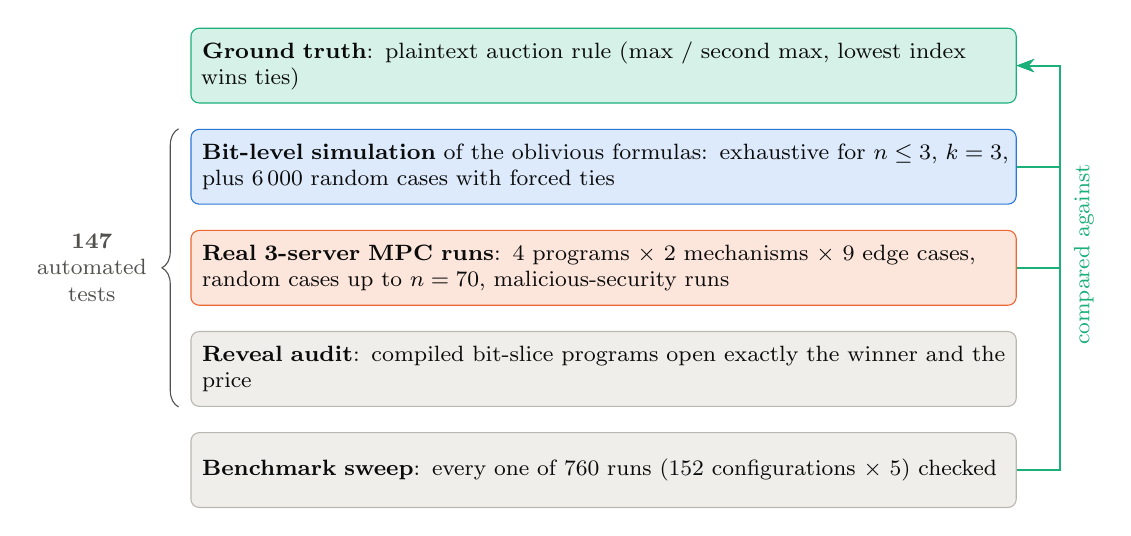
\begin{tikzpicture}[node distance=0.32cm]
  \tikzset{layer/.style={box, text width=10.2cm, align=left, font=\footnotesize, minimum height=0.95cm}}
  \node[layer, fill=vaquabg, draw=vaqua] (l1)
    {\textbf{Ground truth}: plaintext auction rule (max / second max, lowest index wins ties)};
  \node[layer, fill=vbluebg, draw=vblue, below=of l1] (l2)
    {\textbf{Bit-level simulation} of the oblivious formulas: exhaustive for $n \le 3$, $k = 3$,
     plus 6\,000 random cases with forced ties};
  \node[layer, fill=vorangebg, draw=vorange, below=of l2] (l3)
    {\textbf{Real 3-server MPC runs}: 4 programs $\times$ 2 mechanisms $\times$ 9 edge cases, random
     cases up to $n = 70$, malicious-security runs};
  \node[layer, fill=vlight, draw=vline, below=of l3] (l4)
    {\textbf{Reveal audit}: compiled bit-slice programs open exactly the winner and the price};
  \node[layer, fill=vlight, draw=vline, below=of l4] (l5)
    {\textbf{Benchmark sweep}: every one of 760 runs (152 configurations $\times$ 5) checked};
  \draw[arr, draw=vaqua] (l2.east) -- ++(0.55,0) |- (l1.east);
  \draw[arr, draw=vaqua] (l3.east) -- ++(0.55,0) |- (l1.east);
  \draw[arr, draw=vaqua] (l5.east) -- ++(0.55,0) |- (l1.east);
  \node[lbl, text=vaqua, rotate=90] at ($(l1.east)+(0.85,-2.4)$) {compared against};
  \draw[decorate, decoration={brace, amplitude=6pt}, draw=vgray]
    ($(l4.south west)+(-0.15,0)$) -- ($(l2.north west)+(-0.15,0)$)
    node[midway, left=8pt, lbl, align=center] {\textbf{147}\\automated\\tests};
\end{tikzpicture}
}
  \caption{Validation strategy: every layer is checked against the plaintext auction rule.}
  \label{fig:validation}
\end{figure}

% ==============================================================================
\section{Evaluation}
\label{sec:eval}

\paragraph{Setup.}
All experiments run the three servers as separate processes on one machine (AMD Ryzen 7 6800H,
8 cores / 16 threads, 14\,GB RAM, Ubuntu 24.04, MP-SPDZ 0.4.3). Bids are uniformly random; each
configuration is repeated 5 times and we report the median local time. Rounds and data are
MP-SPDZ's per-server figures (the protocols are symmetric) and include preprocessing. Because
localhost has almost no latency, we also report a \emph{modelled} time
\[
  T = T_\text{local} + \text{rounds} \times \text{RTT} + \text{bytes} / \text{bandwidth}
\]
for a LAN (1\,ms RTT, 1\,Gbit/s) and a WAN (50\,ms RTT, 100\,Mbit/s). Rounds and data are measured;
only the network is modelled. We compare four variants: bit-slice and tournament, each in both
domains.

\subsection{The cost model is exact}

Counting operations in \cref{alg:scan} gives $k(3n-1)$ ANDs and $k(\lceil\log_2 n\rceil + 2)$
rounds per scan. The tie-break adds $P(n) + n$ ANDs, where
$P(n) = \sum_{d = 1, 2, 4, \ldots < n} (n - d)$ is the cost of the prefix product. Vickrey adds the
$nk$ ANDs that zero the winner and a second scan. \Cref{tab:model} compares these predictions with
MP-SPDZ's compiler: they agree exactly, in both domains.

\begin{table}[H]
\centering\small
\begin{tabular}{@{}rrlrrr@{}}
\toprule
$n$ & $k$ & mechanism & predicted ANDs & compiled (arithmetic) & compiled (binary) \\
\midrule
3   & 4  & Vickrey & 82     & 82     & 82 \\
5   & 8  & Vickrey & 277    & 277    & 277 \\
128 & 32 & first   & 13\,153 & 13\,153 & 13\,153 \\
128 & 32 & Vickrey & 29\,505 & 29\,505 & 29\,505 \\
256 & 32 & Vickrey & 59\,329 & 59\,329 & 59\,329 \\
\bottomrule
\end{tabular}
\caption{Predicted versus compiled AND counts. Example: for $n=128$, $k=32$, first-price,
$32 \cdot 383 + P(128) + 128 = 12\,256 + 769 + 128 = 13\,153$.}
\label{tab:model}
\end{table}

\subsection{Scaling with the number of bidders and the bid length}

\Cref{fig:scale-n} shows rounds and data as $n$ grows from 2 to 256 with $k = 32$. All variants
grow linearly in data. The bit-slice rounds grow by about $k = 32$ per doubling of $n$, exactly the
$k\lceil\log_2 n\rceil$ term, while the tournament adds only about 10 rounds per doubling.
\Cref{tab:scale-k} isolates the bid length: the bit-slice scan is sequential in $k$, so its rounds
grow linearly, whereas the tournament's rounds stop growing at all beyond $k = 32$ because
MP-SPDZ's comparison needs only $O(\log k)$ rounds.

\begin{figure}[t]
  \centering
  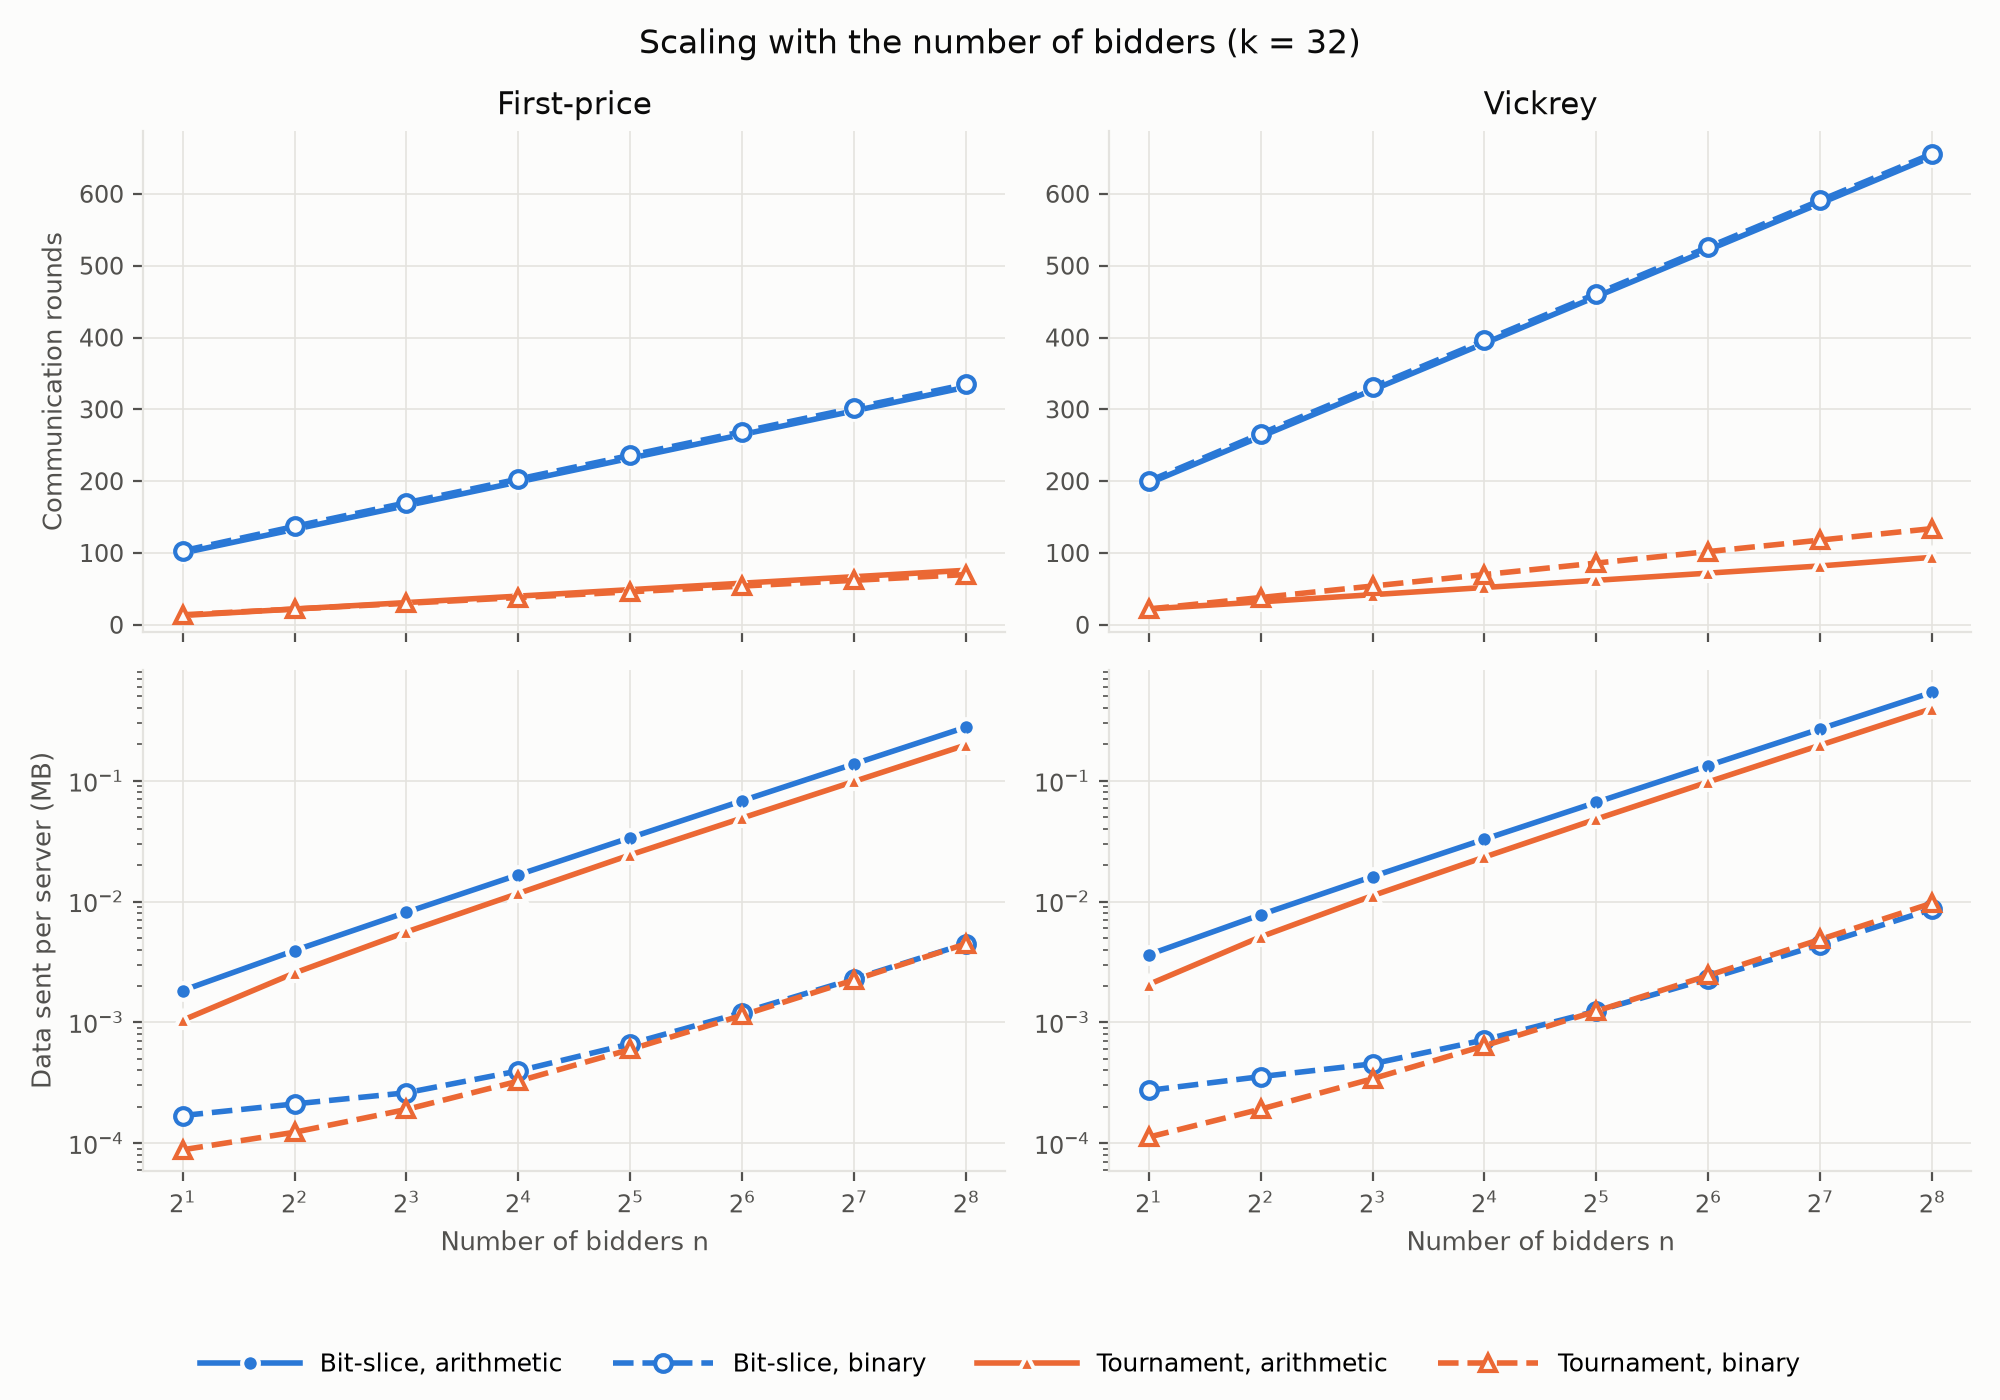
\includegraphics[width=\linewidth]{../bench/results/fig_scale_n.png}
  \caption{Rounds (top) and data per server (bottom, log scale) against the number of bidders,
           $k = 32$. Colour: algorithm; dashed lines with hollow markers: binary domain.}
  \label{fig:scale-n}
\end{figure}

\begin{table}[t]
\centering\small
\begin{tabular}{@{}lrrr@{}}
\toprule
rounds, Vickrey, $n = 32$ & $k = 8$ & $k = 32$ & $k = 60$ \\
\midrule
Bit-slice, arithmetic   & 121 & 457 & 849 \\
Bit-slice, binary       & 125 & 461 & 853 \\
Tournament, arithmetic  & 50  & 62  & 62  \\
Tournament, binary      & 66  & 86  & 86  \\
\bottomrule
\end{tabular}
\caption{Rounds against the bid length. The bit-slice scan is linear in $k$; the comparison-based
tournament is not.}
\label{tab:scale-k}
\end{table}

\subsection{Arithmetic versus binary domain}

\Cref{tab:main} lists every variant at $n = 128$, $k = 32$. Moving the bit-slice circuit to the
binary domain leaves its AND count and rounds unchanged but cuts its data from 0.269\,MB to
0.0044\,MB per server, a $61\times$ reduction. The same move helps the tournament just as much
(0.197\,MB to 0.0049\,MB). Within the binary domain, bit-slice needs 14\% fewer ANDs than the
tournament (29\,505 vs.\ 34\,163) and about 10\% less data; for small $n$ the tournament is slightly
lighter.

\begin{table}[t]
\centering\small
\setlength{\tabcolsep}{5pt}
\begin{tabular}{@{}lrrrrrrr@{}}
\toprule
Variant (Vickrey) & ANDs & rand.\ bits & rounds & MB/server & local (ms) & LAN (s) & WAN (s) \\
\midrule
Bit-slice, arithmetic          & 29\,505 & 0     & 587 & 0.2688 & 19.4 & 0.61 & 29.4 \\
Tournament, arithmetic         & 15\,621 & 8\,636 & 82  & 0.1972 & 5.1  & 0.09 & 4.1 \\
Bit-slice, binary              & 29\,505 & 0     & 591 & 0.0044 & 18.2 & 0.61 & 29.6 \\
Tournament, binary             & 34\,163 & 0     & 118 & 0.0049 & 4.3  & 0.12 & 5.9 \\
\bottomrule
\end{tabular}
\caption{All variants at $n = 128$, $k = 32$, Vickrey. LAN and WAN times are modelled from the
measured rounds and data. First-price costs about half (e.g.\ bit-slice arithmetic: 13\,153 ANDs,
298 rounds, 0.138\,MB).}
\label{tab:main}
\end{table}

\begin{figure}[t]
  \centering
  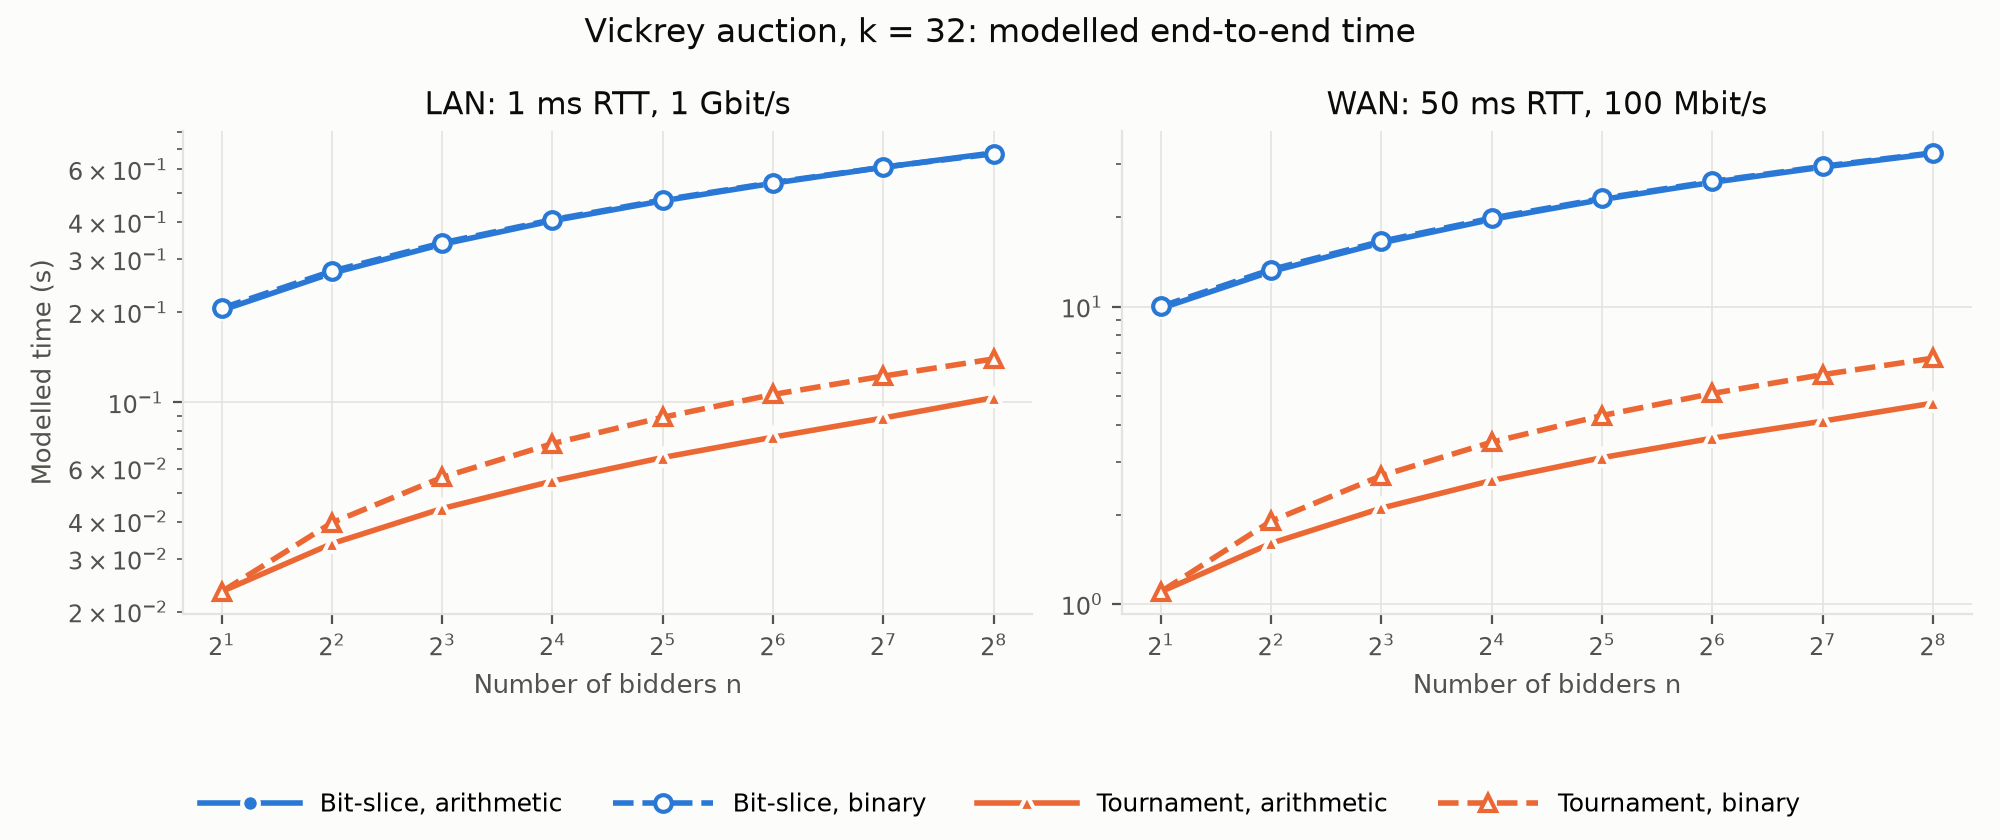
\includegraphics[width=\linewidth]{../bench/results/fig_wan.png}
  \caption{Modelled end-to-end time on a LAN and a WAN (Vickrey, $k = 32$, log scale).}
  \label{fig:wan}
\end{figure}

\subsection{Modelled network time}

On a real network, rounds dominate (\cref{fig:wan}). With 50\,ms of latency the bit-slice auction
over 128 bidders takes about 29\,s against 4--6\,s for the tournament; even on a 1\,ms LAN it takes
0.61\,s against 0.09--0.12\,s. The two bit-slice lines coincide: once data is this small, the
domain no longer matters for time, only the rounds do.

\subsection{Cost of malicious security}
\label{sec:security-eval}

All four programs run unchanged under MP-SPDZ's malicious protocols (\cref{fig:security}). In the
arithmetic domain, communication grows by a factor of about 6 (bit-slice at $n = 64$:
0.134\,MB to 0.823\,MB), with few extra rounds. In the binary domain, the malicious cost is almost
constant at about 0.11--0.13\,MB per server over the sizes we tested, because it is dominated by
MP-SPDZ generating and checking multiplication triples in large fixed batches, not by the circuit.

\begin{figure}[t]
  \centering
  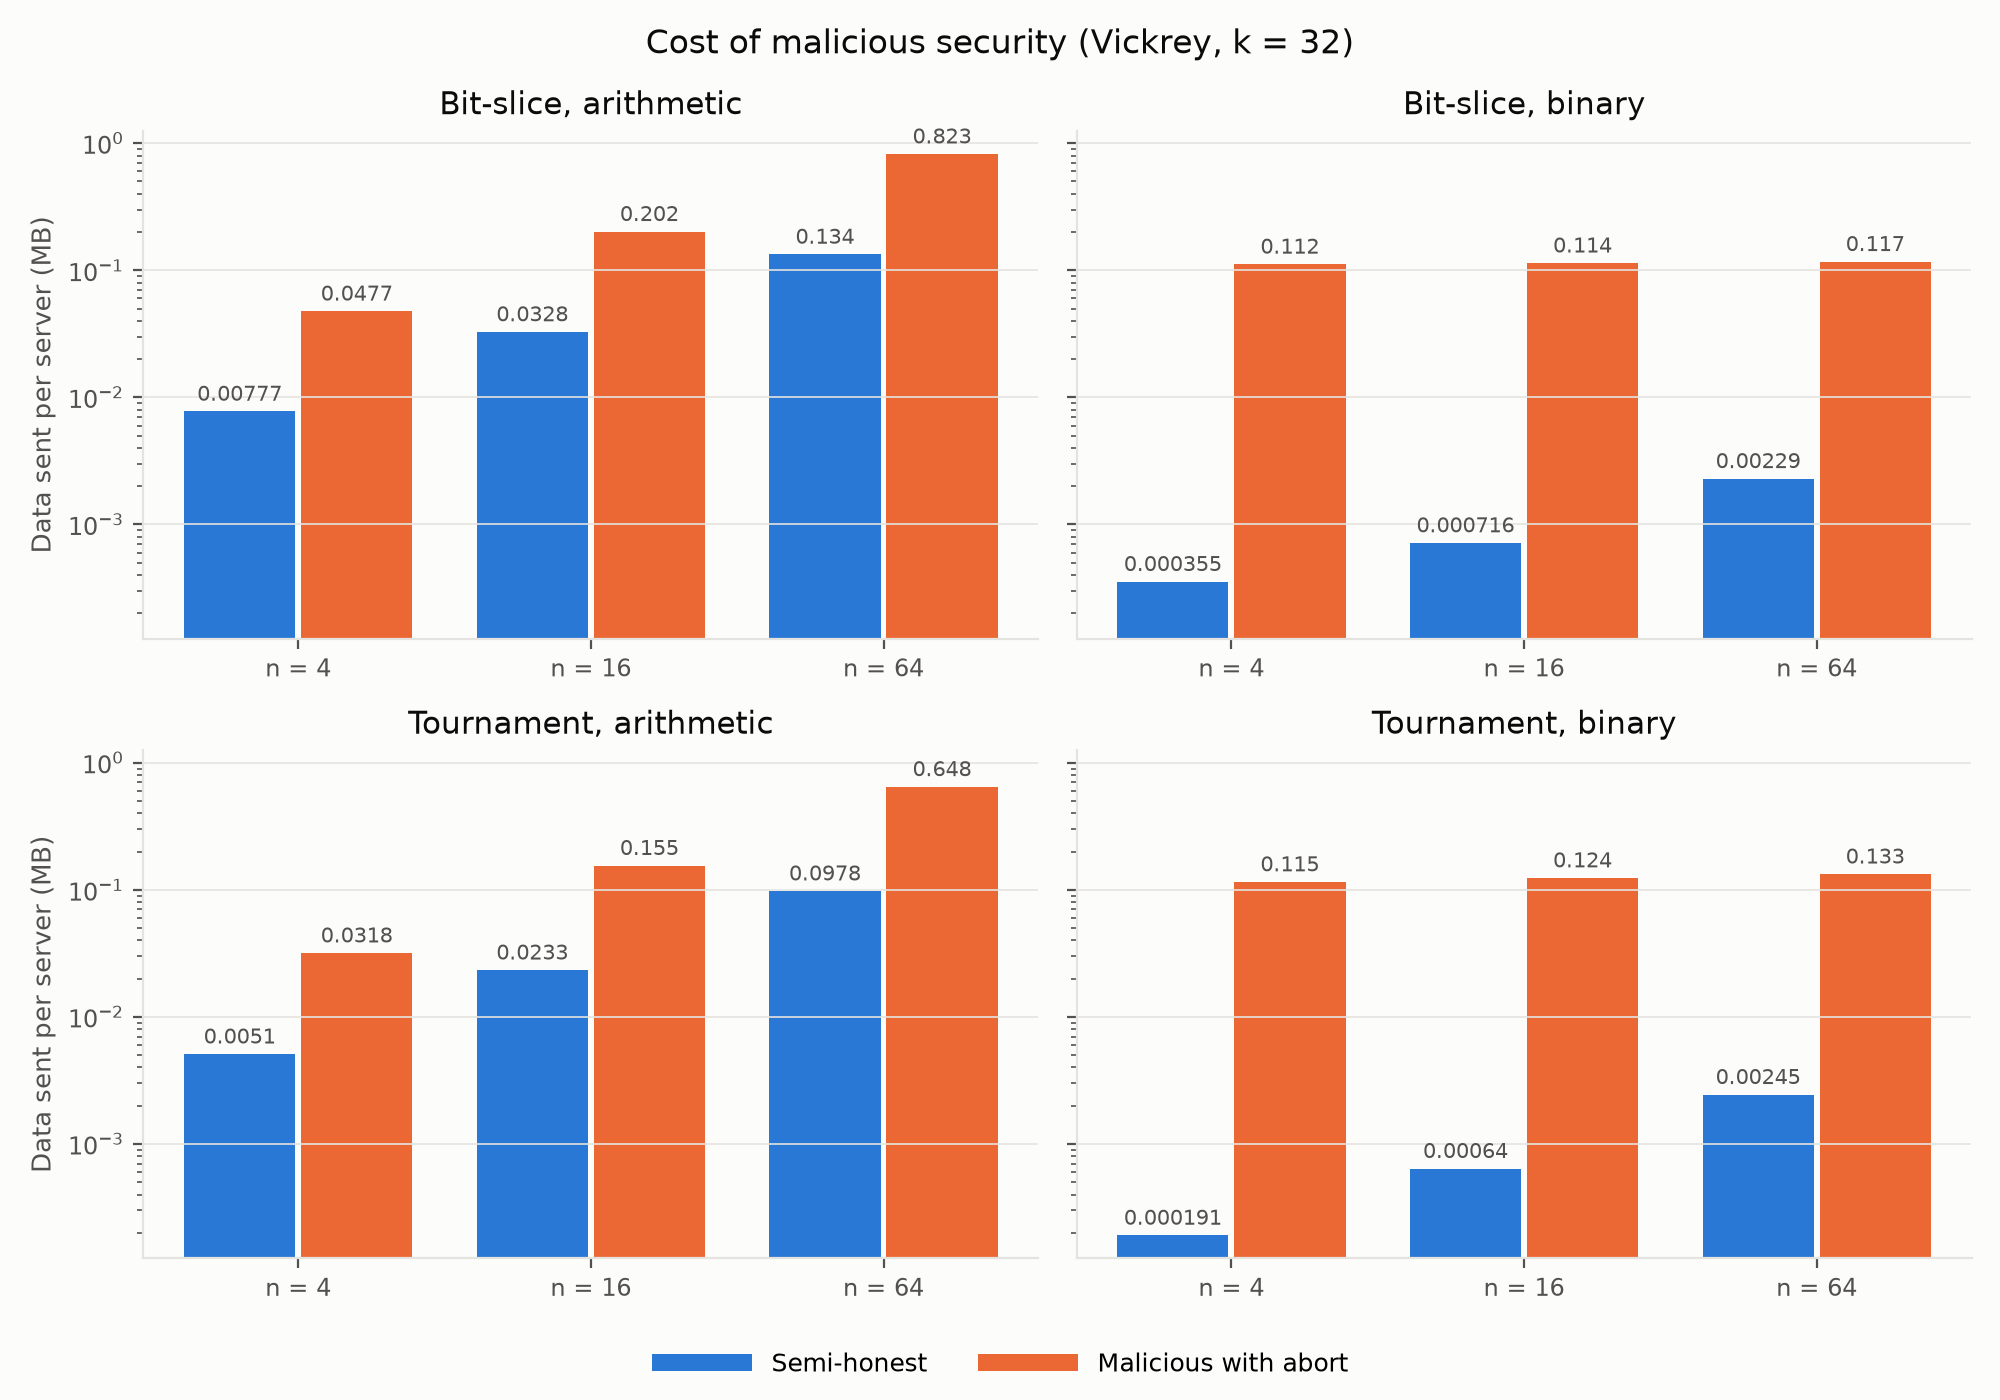
\includegraphics[width=0.92\linewidth]{../bench/results/fig_security.png}
  \caption{Data per server, semi-honest versus malicious security with abort (Vickrey, $k = 32$).}
  \label{fig:security}
\end{figure}

% ==============================================================================
\section{Discussion}
\label{sec:discussion}

\paragraph{Why the baseline wins.}
The survey (\S5.4) argued that the bit-slice scan beats a tournament of comparisons on constants
and round complexity, and Kurosawa and Ogata report a $7\times$ speed-up over the best construction
of their time. Our measurements do not support this on modern MPC. The scan has an inherent
sequential dependency: bit $j - 1$ cannot be processed before the mask from bit $j$ is known,
giving $\Theta(k \log n)$ rounds. MP-SPDZ's comparison uses preprocessed random bits and takes
$O(\log k)$ rounds, so the tournament needs $O(\log n \cdot \log k)$. The claimed advantage was
relative to comparison protocols of 2002, which needed far more rounds than today's.

\paragraph{Where bit-slice still has an edge.}
In the binary domain it needs the fewest ANDs and the least data for large $n$; it opens exactly
two values, whereas the tournament opens $2n$ masked values inside its comparisons; it needs no
comparison sub-protocol or preprocessed random bits, only multiplication; and the same scan carries
over to very different trust models, such as the auctioneer-free SEAL protocol~\cite{seal}, where
comparisons are not available. In a setting where bandwidth is the bottleneck and latency is
negligible, binary bit-slice is the cheapest option we measured.

\paragraph{Domain matters more than algorithm.}
Choosing the binary domain changes communication by $61\times$; choosing between the two
algorithms within one domain changes it by about 10\%. For any boolean-heavy MPC workload, the
domain is the first design decision to make.

\paragraph{Corrections to the literature survey.}
\begin{itemize}
  \item Table~1 printed the mask after bits 1 and 0 as $\{\}$; it should be $\{B\}$
        (\cref{fig:worked}).
  \item \S5.2 describes the update as a branch on the check bit. A secure implementation must be
        branch-free; \cref{eq:update} gives the oblivious form.
  \item \S5.4's round-complexity argument holds against 2002-era comparisons but not against
        modern ones, as discussed above.
\end{itemize}

% ==============================================================================
\section{Limitations and Future Work}

\begin{itemize}
  \item \textbf{Malicious servers and input integrity.} The computation runs under malicious
        security, but bidder inputs should be authenticated, for example with MP-SPDZ's client
        interface, so that a server cannot substitute a share.
  \item \textbf{Public verifiability.} As surveyed in \S6, commitments and zero-knowledge proofs
        (as in Galal and Youssef~\cite{galal}) could let anyone verify the outcome; combining this
        with input privacy remains open in our system.
  \item \textbf{Fewer rounds for bit-slice.} Processing $r$ bits per step (a radix-$2^r$ scan)
        would divide the $k$ term in the round count by $r$ at the price of more ANDs per step.
  \item \textbf{More servers and real networks.} Shamir sharing with more servers would tolerate
        more corruptions; a deployment across real machines would replace our modelled network
        times with measured ones.
  \item \textbf{Auctioneer-free variant.} Implementing the scan with the SEAL protocol~\cite{seal}
        would remove the servers altogether.
\end{itemize}

% ==============================================================================
\section{Individual Contributions}

The work was divided into the four components declared in the mid-term report.

\begin{description}[style=nextline, leftmargin=1.2em]
  \item[Aarav Oswal (230012): computation environment and testing]
        Installation and configuration of MP-SPDZ for the 3-server setting, including Windows
        support through WSL2 (\code{setup/}); the runner that compiles programs, launches the
        servers and parses their output (\code{runner.py}); the plaintext reference and bit-level
        simulation (\code{reference.py}); and the 147-test suite that validates every component
        against the reference.
  \item[Ch.\ Rishitha (230311): bit-slice maximum circuit]
        The oblivious bit-slice scan in both domains (\code{auction.mpc}, \code{auction\_bin.mpc}):
        the branch-free mask update, the log-depth OR tree, the oblivious lowest-index tie-break,
        and the extraction of the maximum from the per-bit OR results.
  \item[R.\ Charan (230819): Vickrey extension and performance evaluation]
        The oblivious second scan for the Vickrey price; the comparison-tournament baselines in
        both domains; the benchmark harness and figures (\code{bench/}); and the analysis of
        scaling, network cost and malicious-security overhead.
  \item[Poorvie Sadagopan (230759): input and output pipeline]
        Bidder-side additive and XOR secret sharing and the server input layout
        (\code{sharing.py}); the output boundary that opens only the winner and price, verified by
        the reveal audit (\code{audit.py}); and the command-line demo (\code{cli.py}).
\end{description}

% ==============================================================================
\section{Conclusion}

We built a privacy-preserving sealed-bid auction in which three servers compute the winner and
the first- or second-price outcome without any of them seeing a bid, opening only the winner and
the price. The bit-slice circuit is simple, oblivious and exactly predictable in cost, and moving
it to the binary domain cuts its communication by $61\times$. Our evaluation also shows that its
sequential dependency on the bid length makes it slower than a modern comparison-based tournament
on any network with real latency, an honest correction to our own survey and a useful lesson about
how far a 2002 efficiency claim carries into today's MPC.

\paragraph{Reproducing the results.}
\code{bash setup/setup.sh} installs everything; \code{.venv/bin/pytest -q} runs the tests;
\code{.venv/bin/python bench/run\_bench.py} and \code{bench/plot.py} regenerate every number and
figure in \cref{sec:eval}. Source code: \url{https://github.com/rcharan05/CS670_Project}.

% ==============================================================================
\begin{thebibliography}{99}\small
\bibitem{araki16} T.~Araki, J.~Furukawa, Y.~Lindell, A.~Nof, K.~Ohara.
  High-throughput semi-honest secure three-party computation with an honest majority.
  In \emph{ACM CCS}, pages 805--817, 2016. doi:10.1145/2976749.2978331.
\bibitem{seal} S.~Bag, F.~Hao, S.~F.~Shahandashti, I.~G.~Ray.
  SEAL: Sealed-bid auction without auctioneers.
  \emph{IEEE TIFS}, 15:2042--2052, 2020. doi:10.1109/TIFS.2019.2955793.
\bibitem{bogetoft06} P.~Bogetoft, I.~Damg{\aa}rd, T.~Jakobsen, K.~Nielsen, J.~Pagter, T.~Toft.
  A practical implementation of secure auctions based on multiparty integer computation.
  In \emph{Financial Cryptography}, LNCS 4107, pages 142--147, 2006. doi:10.1007/11889663\_10.
\bibitem{bogetoft09} P.~Bogetoft, D.~L.~Christensen, I.~Damg{\aa}rd, M.~Geisler, T.~Jakobsen,
  M.~Kr{\o}igaard, J.~D.~Nielsen, J.~B.~Nielsen, K.~Nielsen, J.~Pagter, M.~Schwartzbach, T.~Toft.
  Secure multiparty computation goes live.
  In \emph{Financial Cryptography}, LNCS 5628, pages 325--343, 2009.
  doi:10.1007/978-3-642-03549-4\_20.
\bibitem{furukawa17} J.~Furukawa, Y.~Lindell, A.~Nof, O.~Weinstein.
  High-throughput secure three-party computation for malicious adversaries and an honest majority.
  In \emph{EUROCRYPT}, 2017.
\bibitem{galal} H.~S.~Galal, A.~M.~Youssef.
  Verifiable sealed-bid auction on the Ethereum blockchain.
  In \emph{Financial Cryptography Workshops}, LNCS 10958, pages 265--278, 2019.
  doi:10.1007/978-3-662-58820-8\_18.
\bibitem{mpspdz} M.~Keller.
  MP-SPDZ: A versatile framework for multi-party computation.
  In \emph{ACM CCS}, pages 1575--1590, 2020. doi:10.1145/3372297.3417872.
\bibitem{ko02} K.~Kurosawa, W.~Ogata.
  Bit-slice auction circuit.
  In \emph{ESORICS}, LNCS 2502, pages 24--38, 2002. doi:10.1007/3-540-45853-0\_2.
\bibitem{lindellnof17} Y.~Lindell, A.~Nof.
  A framework for constructing fast MPC over arithmetic circuits with malicious adversaries and an
  honest-majority. In \emph{ACM CCS}, 2017.
\bibitem{nps99} M.~Naor, B.~Pinkas, R.~Sumner.
  Privacy preserving auctions and mechanism design.
  In \emph{ACM EC}, pages 129--139, 1999. doi:10.1145/336992.337028.
\end{thebibliography}

\end{document}
